

\clearpage
\subsection{The Leather merchant}
\label{sec:appendix:moj:leather}

Viking leather workers made shoes for those who could afford them. To own a pair of shoes was a status symbol and showed that you had wealth. They also made bags, belts and scabbards for swords.

\begin{display}{The leather stall}
	\label{fig:appendix:moj:places:leather:stall}
	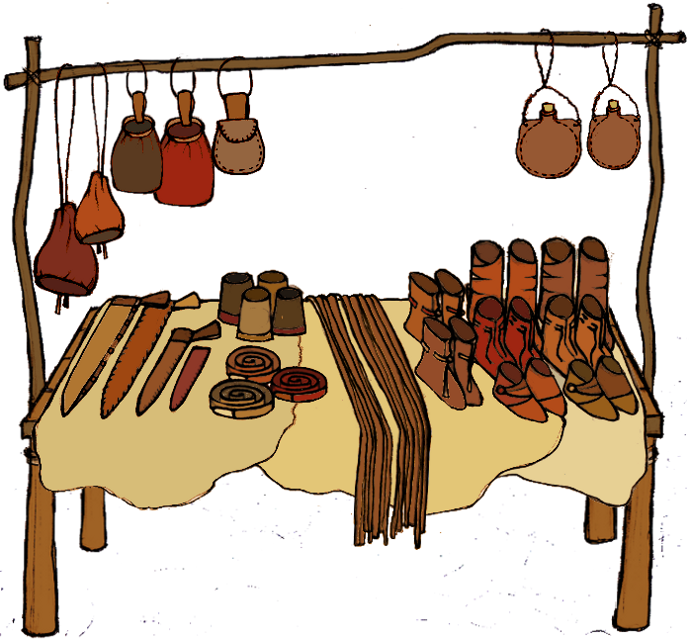
\includegraphics[width=0.65\columnwidth]{img/Jorvik/places/leather stall}
\end{display}

\begin{display}{The leather stall with a background and a merchant}
	\label{fig:appendix:moj:places:leather}
	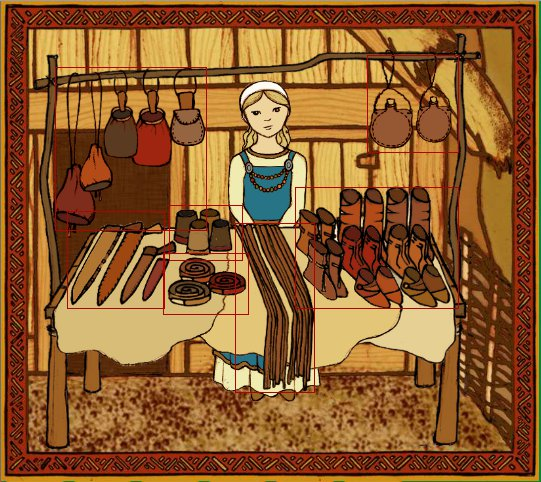
\includegraphics[width=0.65\columnwidth]{img/Jorvik/places/leather}
\end{display}
\clearpage


\begin{table}[ht!]
	\centering
	\begin{tabular}{ p{3cm} c }\toprule
		\textbf{Name:} & \multirow{5}{*}{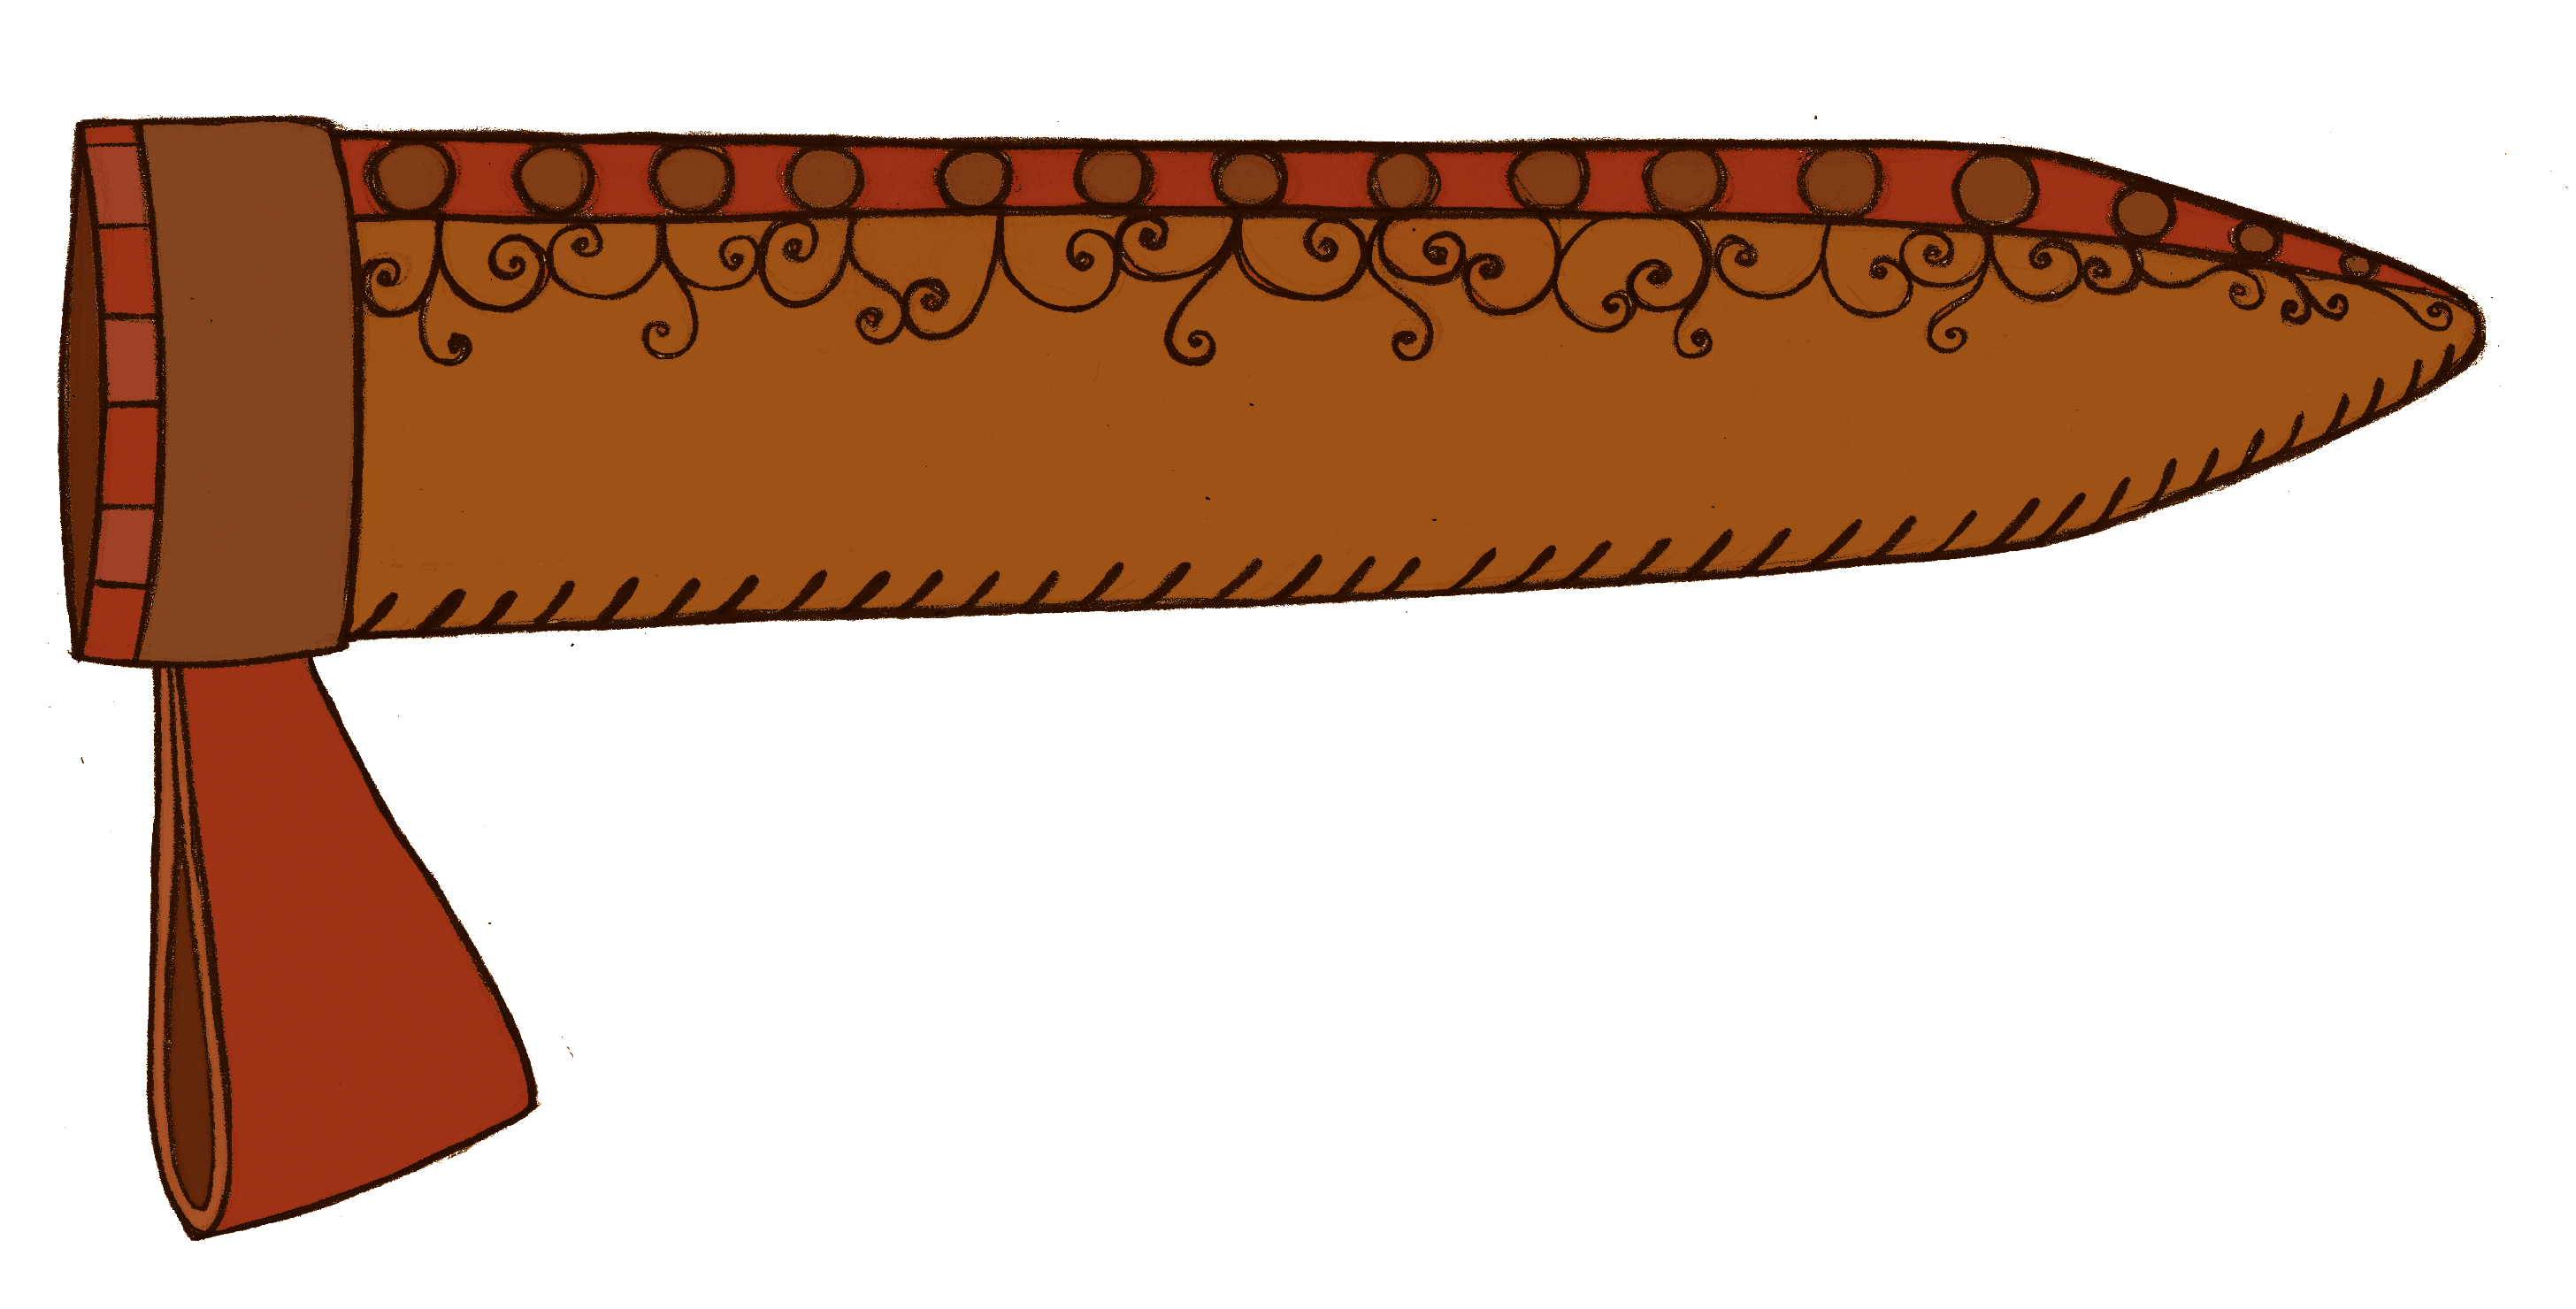
\includegraphics[height=30mm]{img/Jorvik/objects/leather/sheath}}\\
		Sheath & \\ 
		\textbf{Price:} & \\
		14.11 silver. & \\ 
		\textbf{Description:} & \\
		\multicolumn{2}{p{12cm}}{When a sword was not in use it was kept safe in its sheath, called a scabbard. They were sometimes lined with fleece or fabric to further protect the blade}\\
		\bottomrule
	\end{tabular}
\end{table}

\begin{table}[ht!]
	\centering
	\begin{tabular}{ p{3cm} c }\toprule
		\textbf{Name:} & \multirow{5}{*}{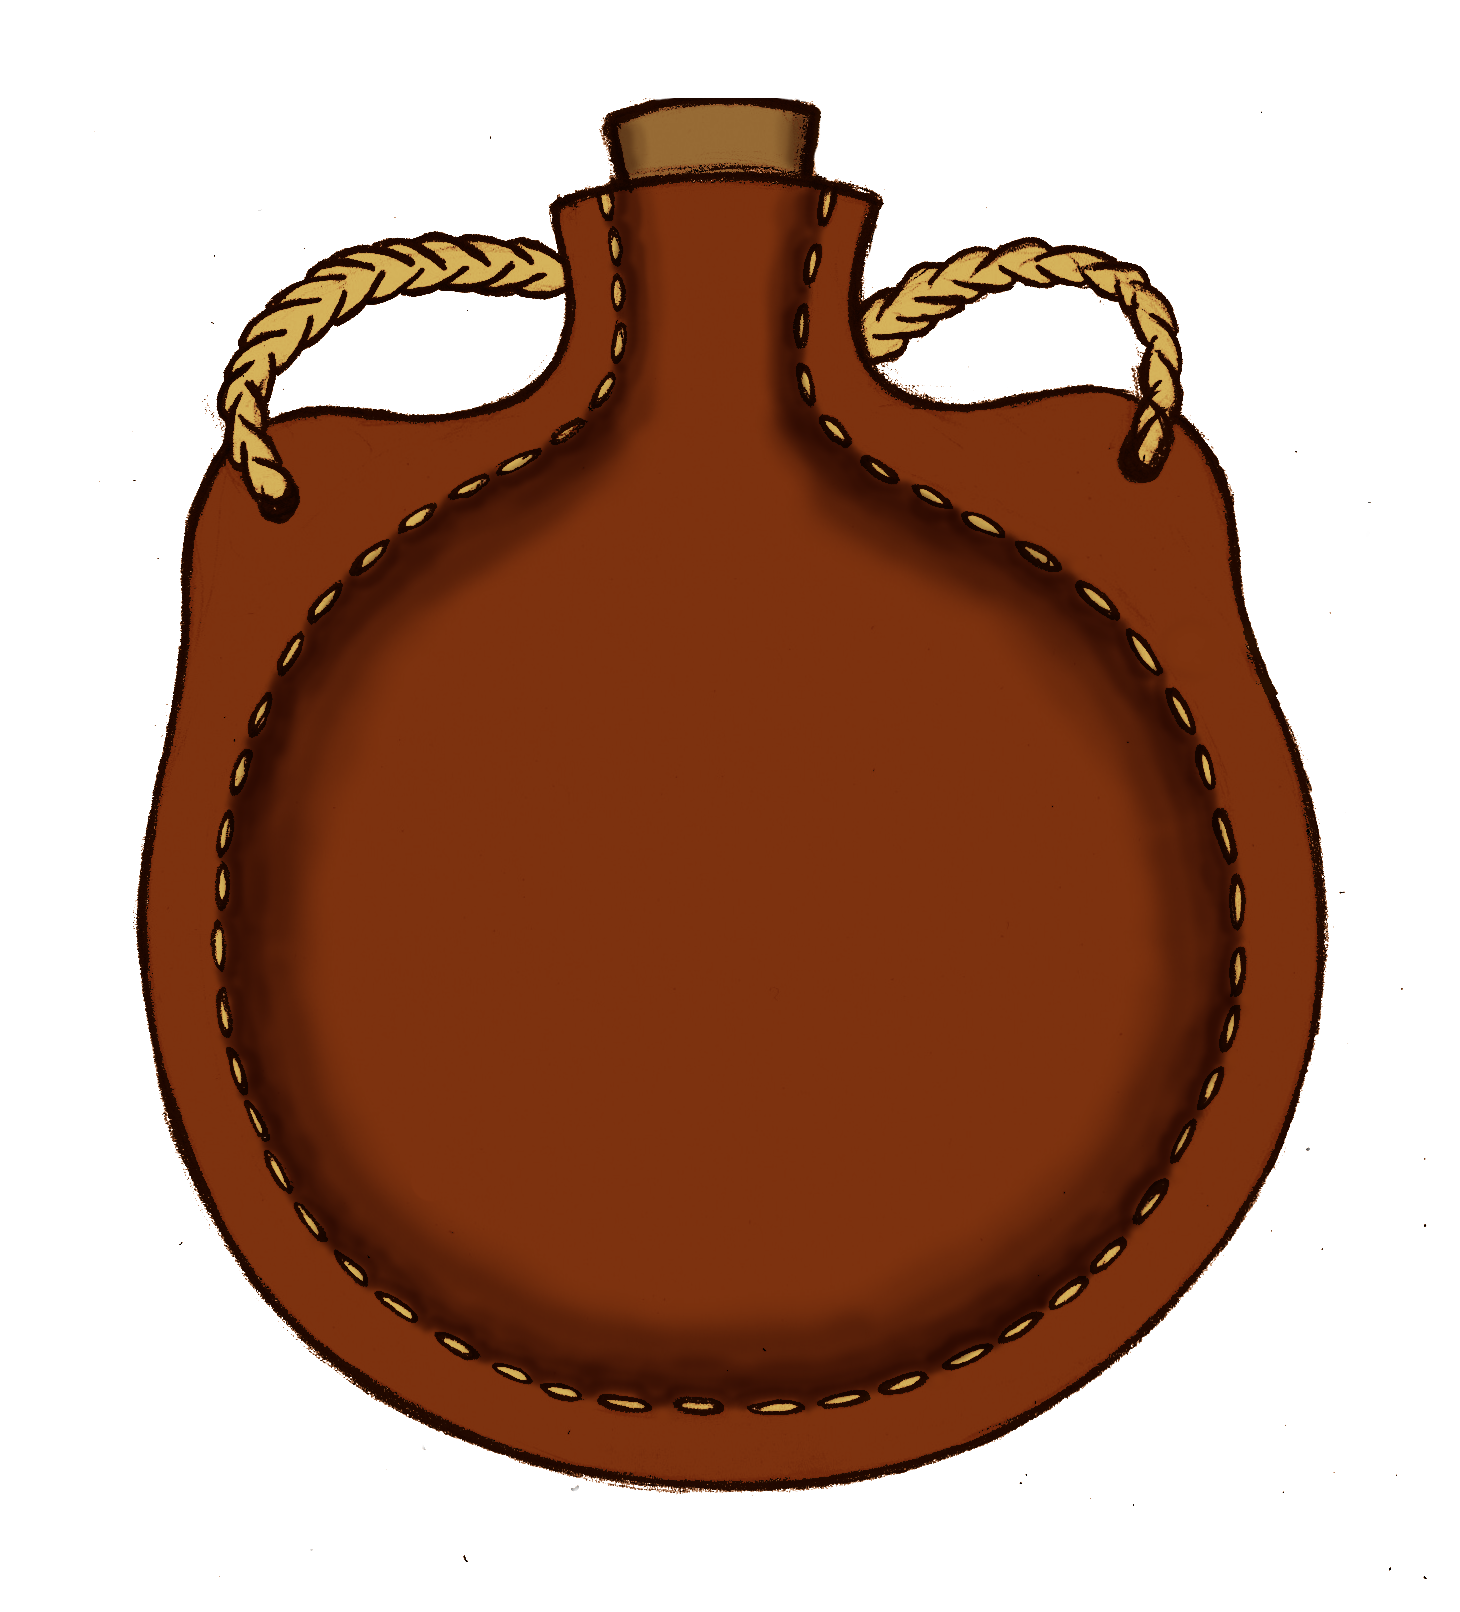
\includegraphics[height=30mm]{img/Jorvik/objects/leather/drinking bottle}}\\
		Drinking Bottle & \\ 
		\textbf{Price:} & \\
		11.03 silver. & \\ 
		\textbf{Description:} & \\
		\multicolumn{2}{p{12cm}}{A bottle, or costrel, used for storing and serving drinks could be made out of leather, wood or clay.}\\
		\bottomrule
	\end{tabular}
\end{table}

\begin{table}[ht!]
	\centering
	\begin{tabular}{ p{3cm} c }\toprule
		\textbf{Name:} & \multirow{5}{*}{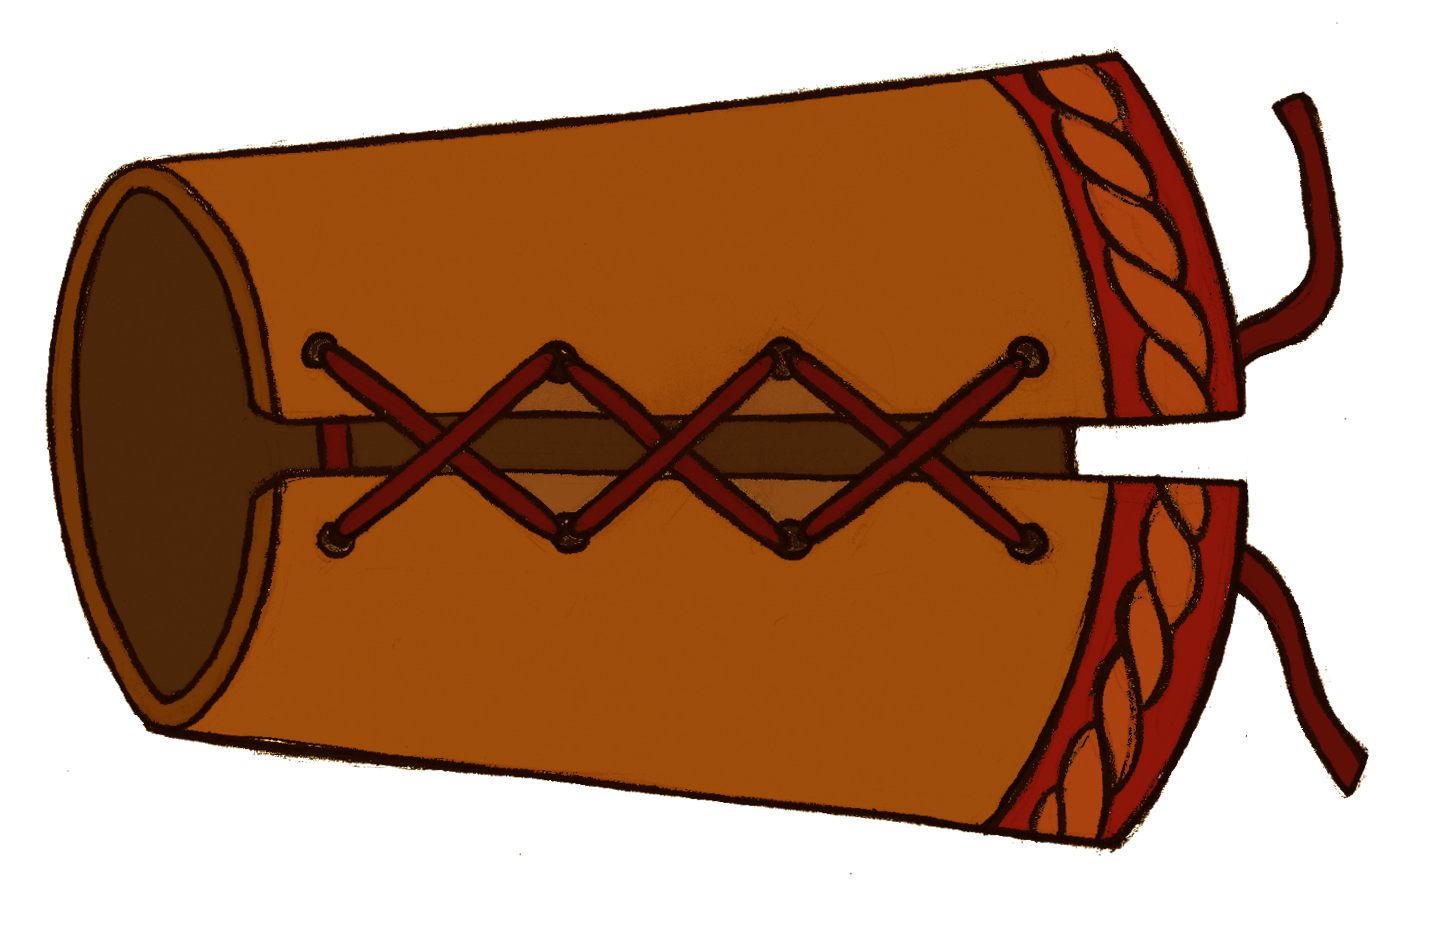
\includegraphics[height=30mm]{img/Jorvik/objects/leather/vambraces}}\\
		Vambraces & \\ 
		\textbf{Price:} & \\
		22.05 silver. & \\ 
		\textbf{Description:} & \\
		\multicolumn{2}{p{12cm}}{Vikings often wore chainmail in battle to protect their body in battle but they needed leather vambraces to give protection to their arms.}\\
		\bottomrule
	\end{tabular}
\end{table}

\begin{table}[ht!]
	\centering
	\begin{tabular}{ p{3cm} c }\toprule
		\textbf{Name:} & \multirow{5}{*}{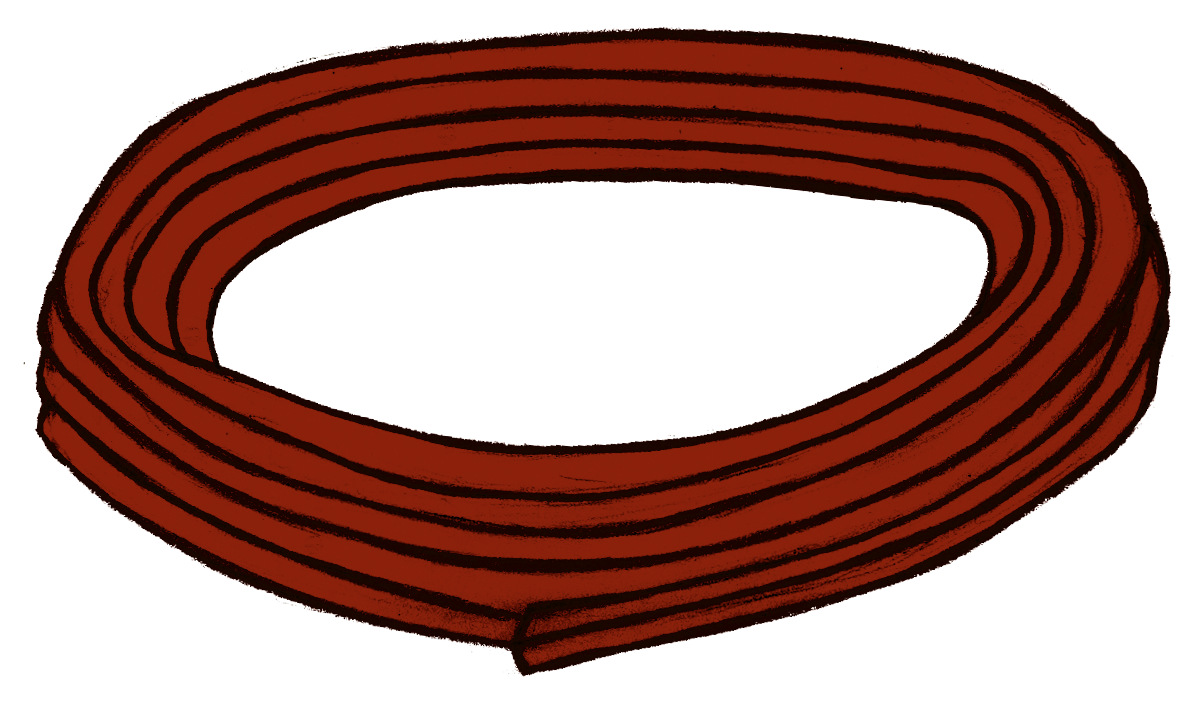
\includegraphics[height=30mm]{img/Jorvik/objects/leather/thong}}\\
		Thong & \\ 
		\textbf{Price:} & \\
		2.21 silver. & \\ 
		\textbf{Description:} & \\
		\multicolumn{2}{p{12cm}}{Leather thongs could be used as a belt or to attach skates to shoes. They were very useful to have around the home.}\\
		\bottomrule
	\end{tabular}
\end{table}

\begin{table}[ht!]
	\centering
	\begin{tabular}{ p{3cm} c }\toprule
		\textbf{Name:} & \multirow{5}{*}{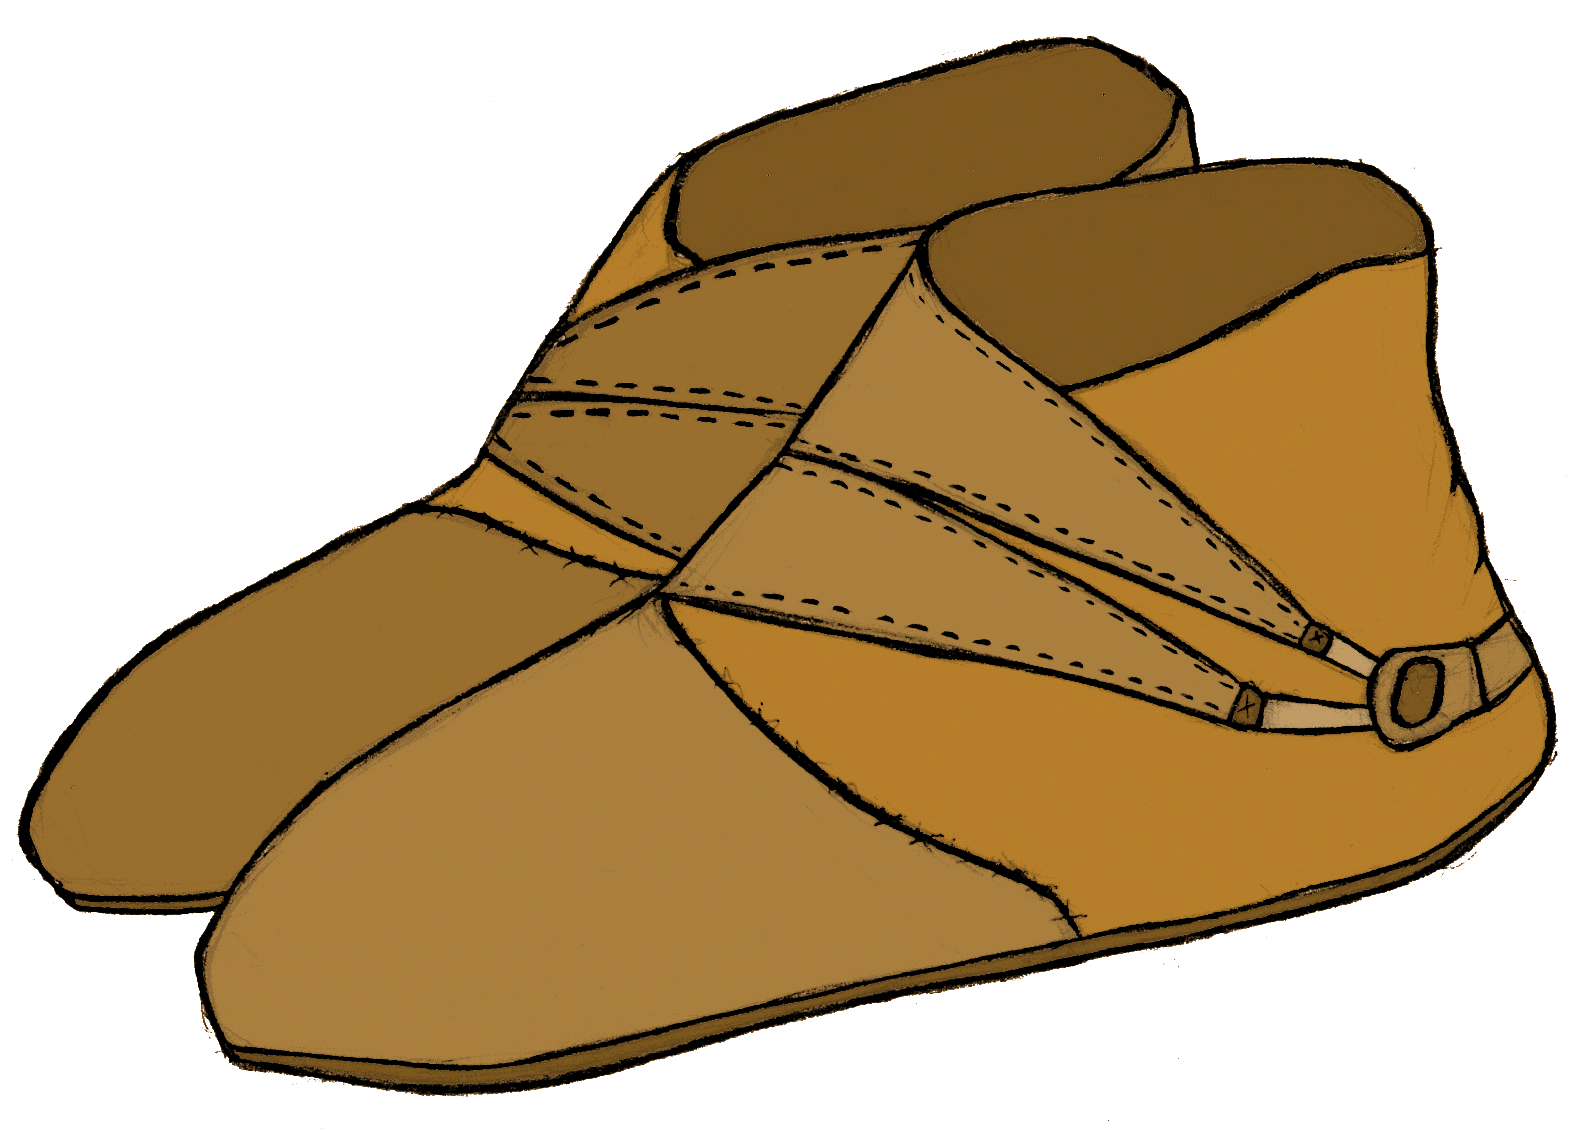
\includegraphics[height=30mm]{img/Jorvik/objects/leather/shoes}}\\
		Shoes & \\ 
		\textbf{Price:} & \\
		26.46 silver. & \\ 
		\textbf{Description:} & \\
		\multicolumn{2}{p{12cm}}{Norse shoes may not have lasted very long so they either underwent many repairs or were replaced regularly. }\\
		\bottomrule
	\end{tabular}
\end{table}

\begin{table}[ht!]
	\centering
	\begin{tabular}{ p{3cm} c }\toprule
		\textbf{Name:} & \multirow{5}{*}{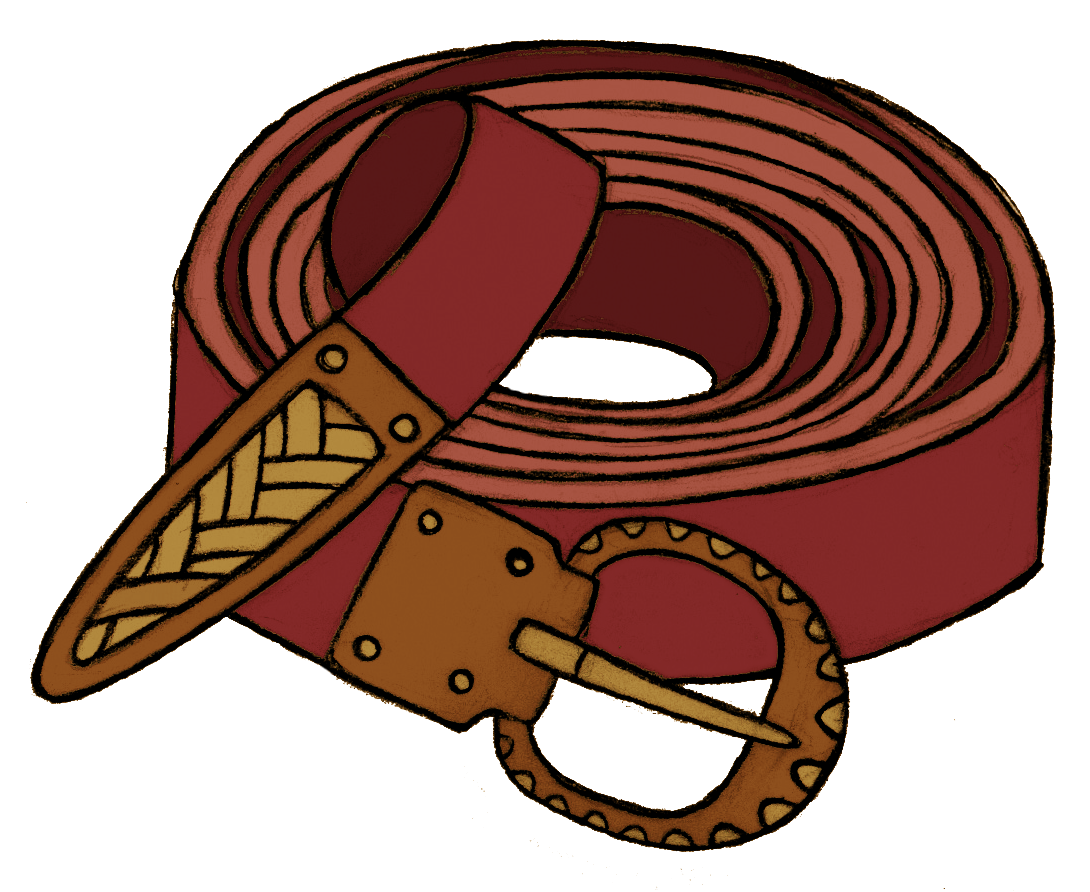
\includegraphics[height=30mm]{img/Jorvik/objects/leather/belt}}\\
		Belt & \\ 
		\textbf{Price:} & \\
		8.82 silver. & \\ 
		\textbf{Description:} & \\
		\multicolumn{2}{p{12cm}}{Belts were made to be about 2cm wide, much narrower than modern belts. Every part of the belt might be decorated, the Coppergate dig have unearthed examples of both decorated and non-decorated belts and buckles.}\\
		\bottomrule
	\end{tabular}
\end{table}

\begin{table}[ht!]
	\centering
	\begin{tabular}{ p{3cm} c }\toprule
		\textbf{Name:} & \multirow{5}{*}{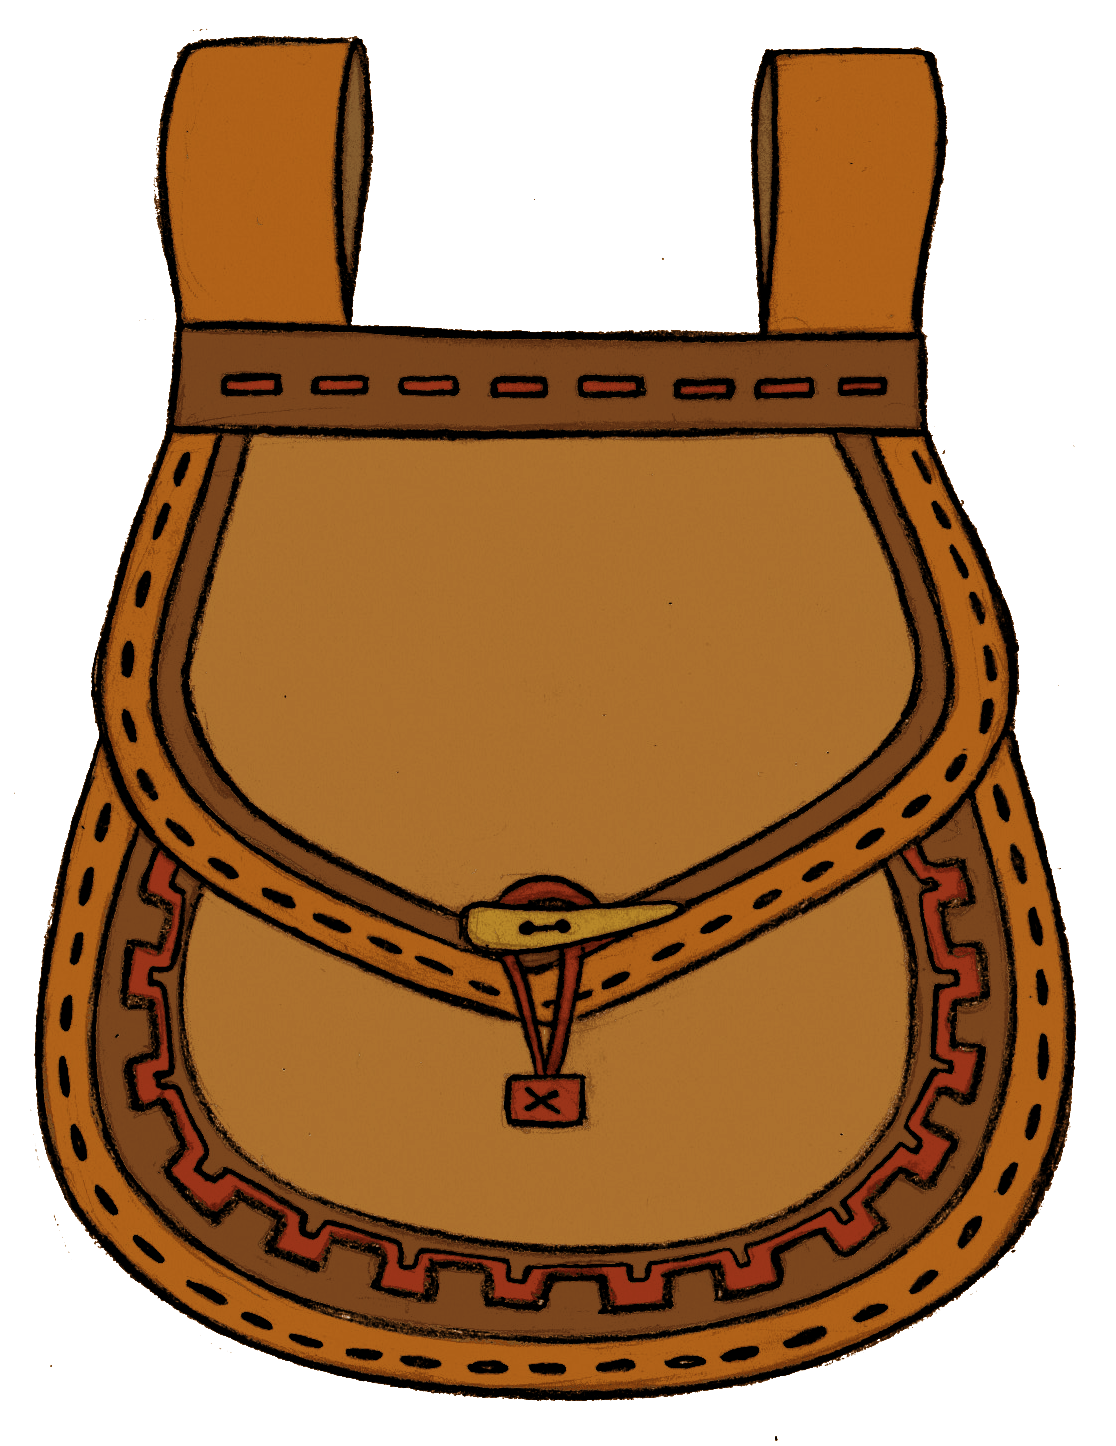
\includegraphics[height=30mm]{img/Jorvik/objects/leather/bag}}\\
		Bag & \\ 
		\textbf{Price:} & \\
		17.64 silver. & \\ 
		\textbf{Description:} & \\
		\multicolumn{2}{p{12cm}}{Viking clothing had no pockets so they used leather bags to carry coins, keys, a clean cloth and other small, useful items. The pouches would hang from their belts.}\\
		\bottomrule
	\end{tabular}
\end{table}